\documentclass[nooutcomes]{ximera}
%% handout
%% space
%% newpage
%% numbers
%% nooutcomes

%I added the commands here so that I would't have to keep looking them up
%\newcommand{\RR}{\mathbb R}
%\renewcommand{\d}{\,d}
%\newcommand{\dd}[2][]{\frac{d #1}{d #2}}
%\renewcommand{\l}{\ell}
%\newcommand{\ddx}{\frac{d}{dx}}
%\everymath{\displaystyle}
%\newcommand{\dfn}{\textbf}
%\newcommand{\eval}[1]{\bigg[ #1 \bigg]}

%\begin{image}
%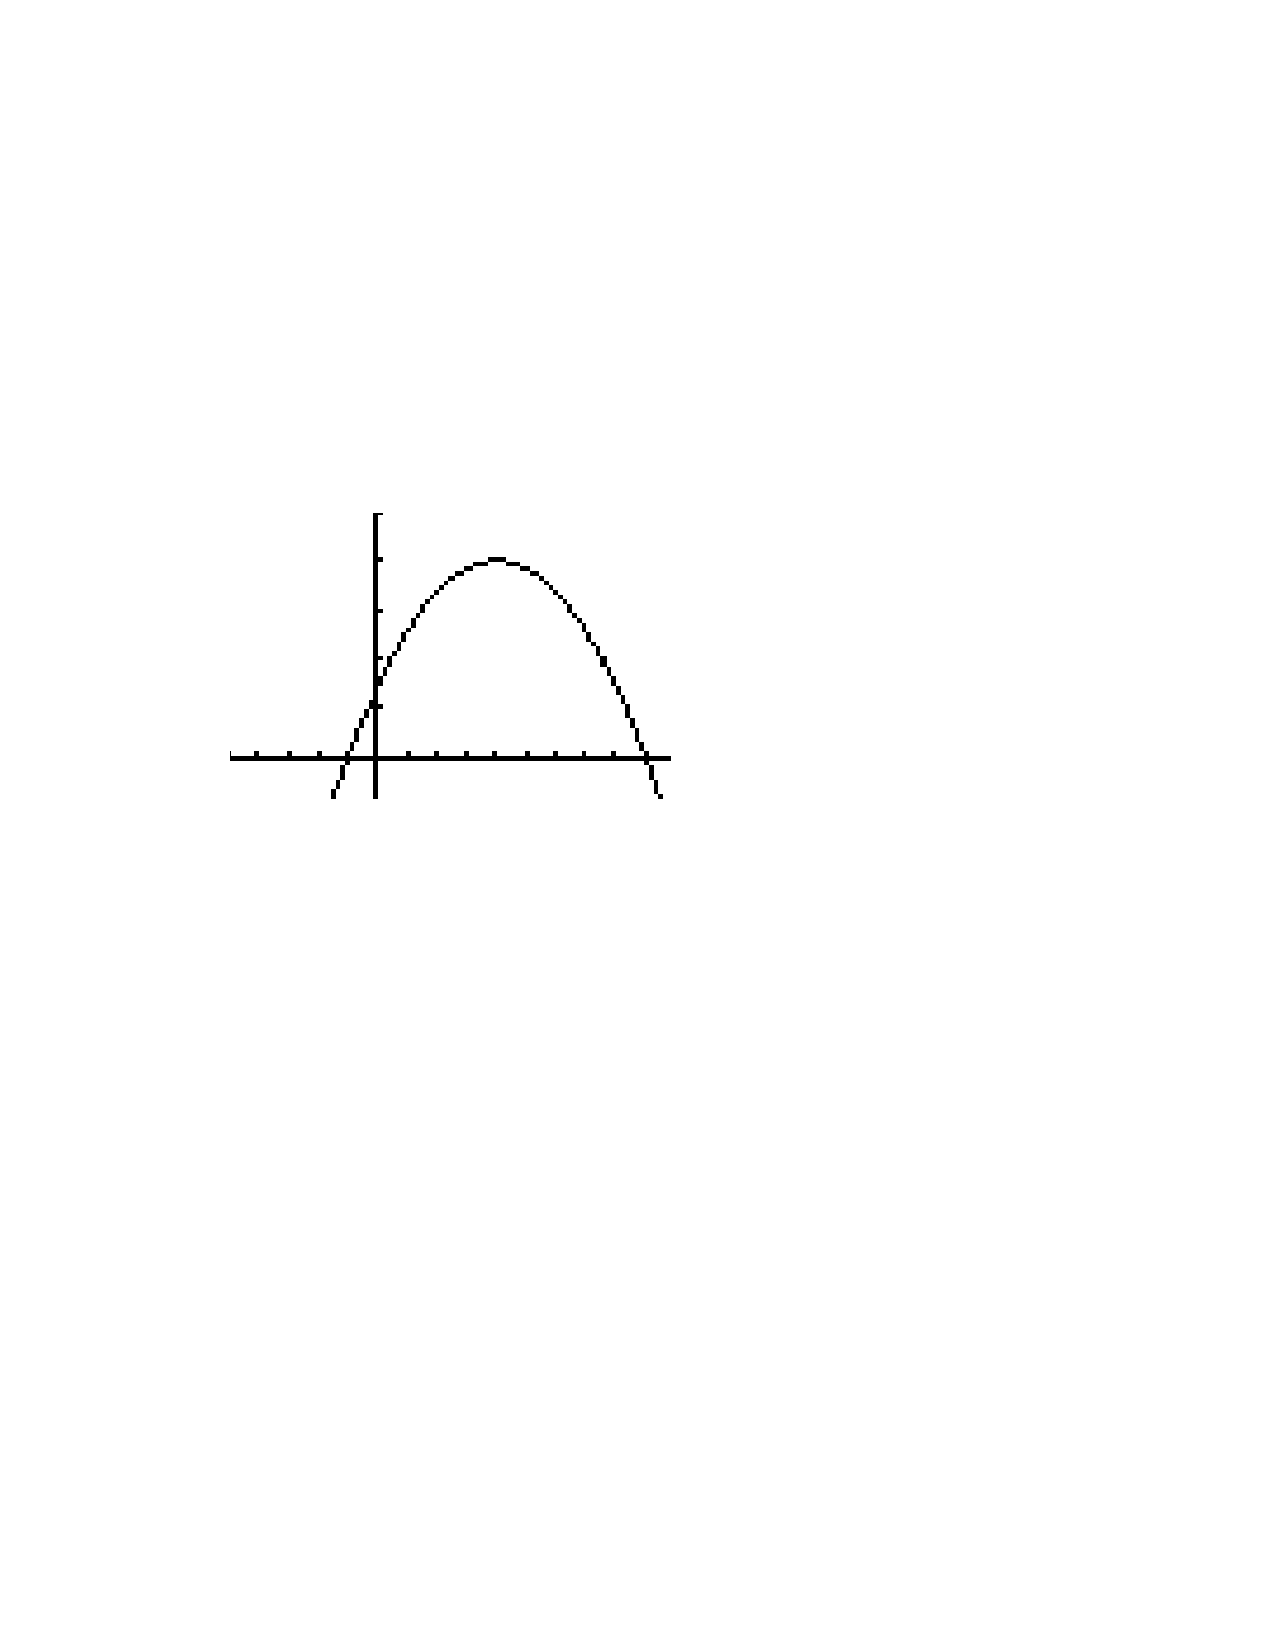
\includegraphics[trim= 170 420 250 180]{Figure1.pdf}
%\end{image}

\usepackage{fullpage}
\newcommand{\RR}{\mathbb R}
\renewcommand{\d}{\,d}
\newcommand{\dd}[2][]{\frac{d #1}{d #2}}
\renewcommand{\l}{\ell}
\newcommand{\ddx}{\frac{d}{dx}}
\newcommand{\dfn}{\textbf}
\newcommand{\eval}[1]{\bigg[ #1 \bigg]}

\usepackage{multicol}

\renewenvironment{freeResponse}{
\ifhandout\setbox0\vbox\bgroup\else
\begin{trivlist}\item[\hskip \labelsep\bfseries Solution:\hspace{2ex}]
\fi}
{\ifhandout\egroup\else
\end{trivlist}
\fi} %% we can turn off input when making a master document

\title{1.3 and 3.9: Derivatives of exponential and logarithmic functions}  

\begin{document}
\begin{abstract}		\end{abstract}
\maketitle

%problem1
\begin{problem}
Explain what each of the following means:

  \begin{enumerate}

    % part a
  \item $f^{-1}(x)$
    \begin{freeResponse}
      This denotes the inverse function of $f(x)$.
    \end{freeResponse}
		
    % part b
  \item $f(x^{-1})$
    \begin{freeResponse}
      This means $f \left( \frac{1}{x} \right)$.
    \end{freeResponse}
		
    % part c
  \item $\left( f(x) \right)^{-1}$
    \begin{freeResponse}
      This means $f(x)$ raised to the $-1$ power,
      i.e. $\frac{1}{f(x)}$.
    \end{freeResponse}
  \end{enumerate}
\end{problem}

%problem2
\begin{problem}

  We're given the following graph of a function:
  \begin{image}
    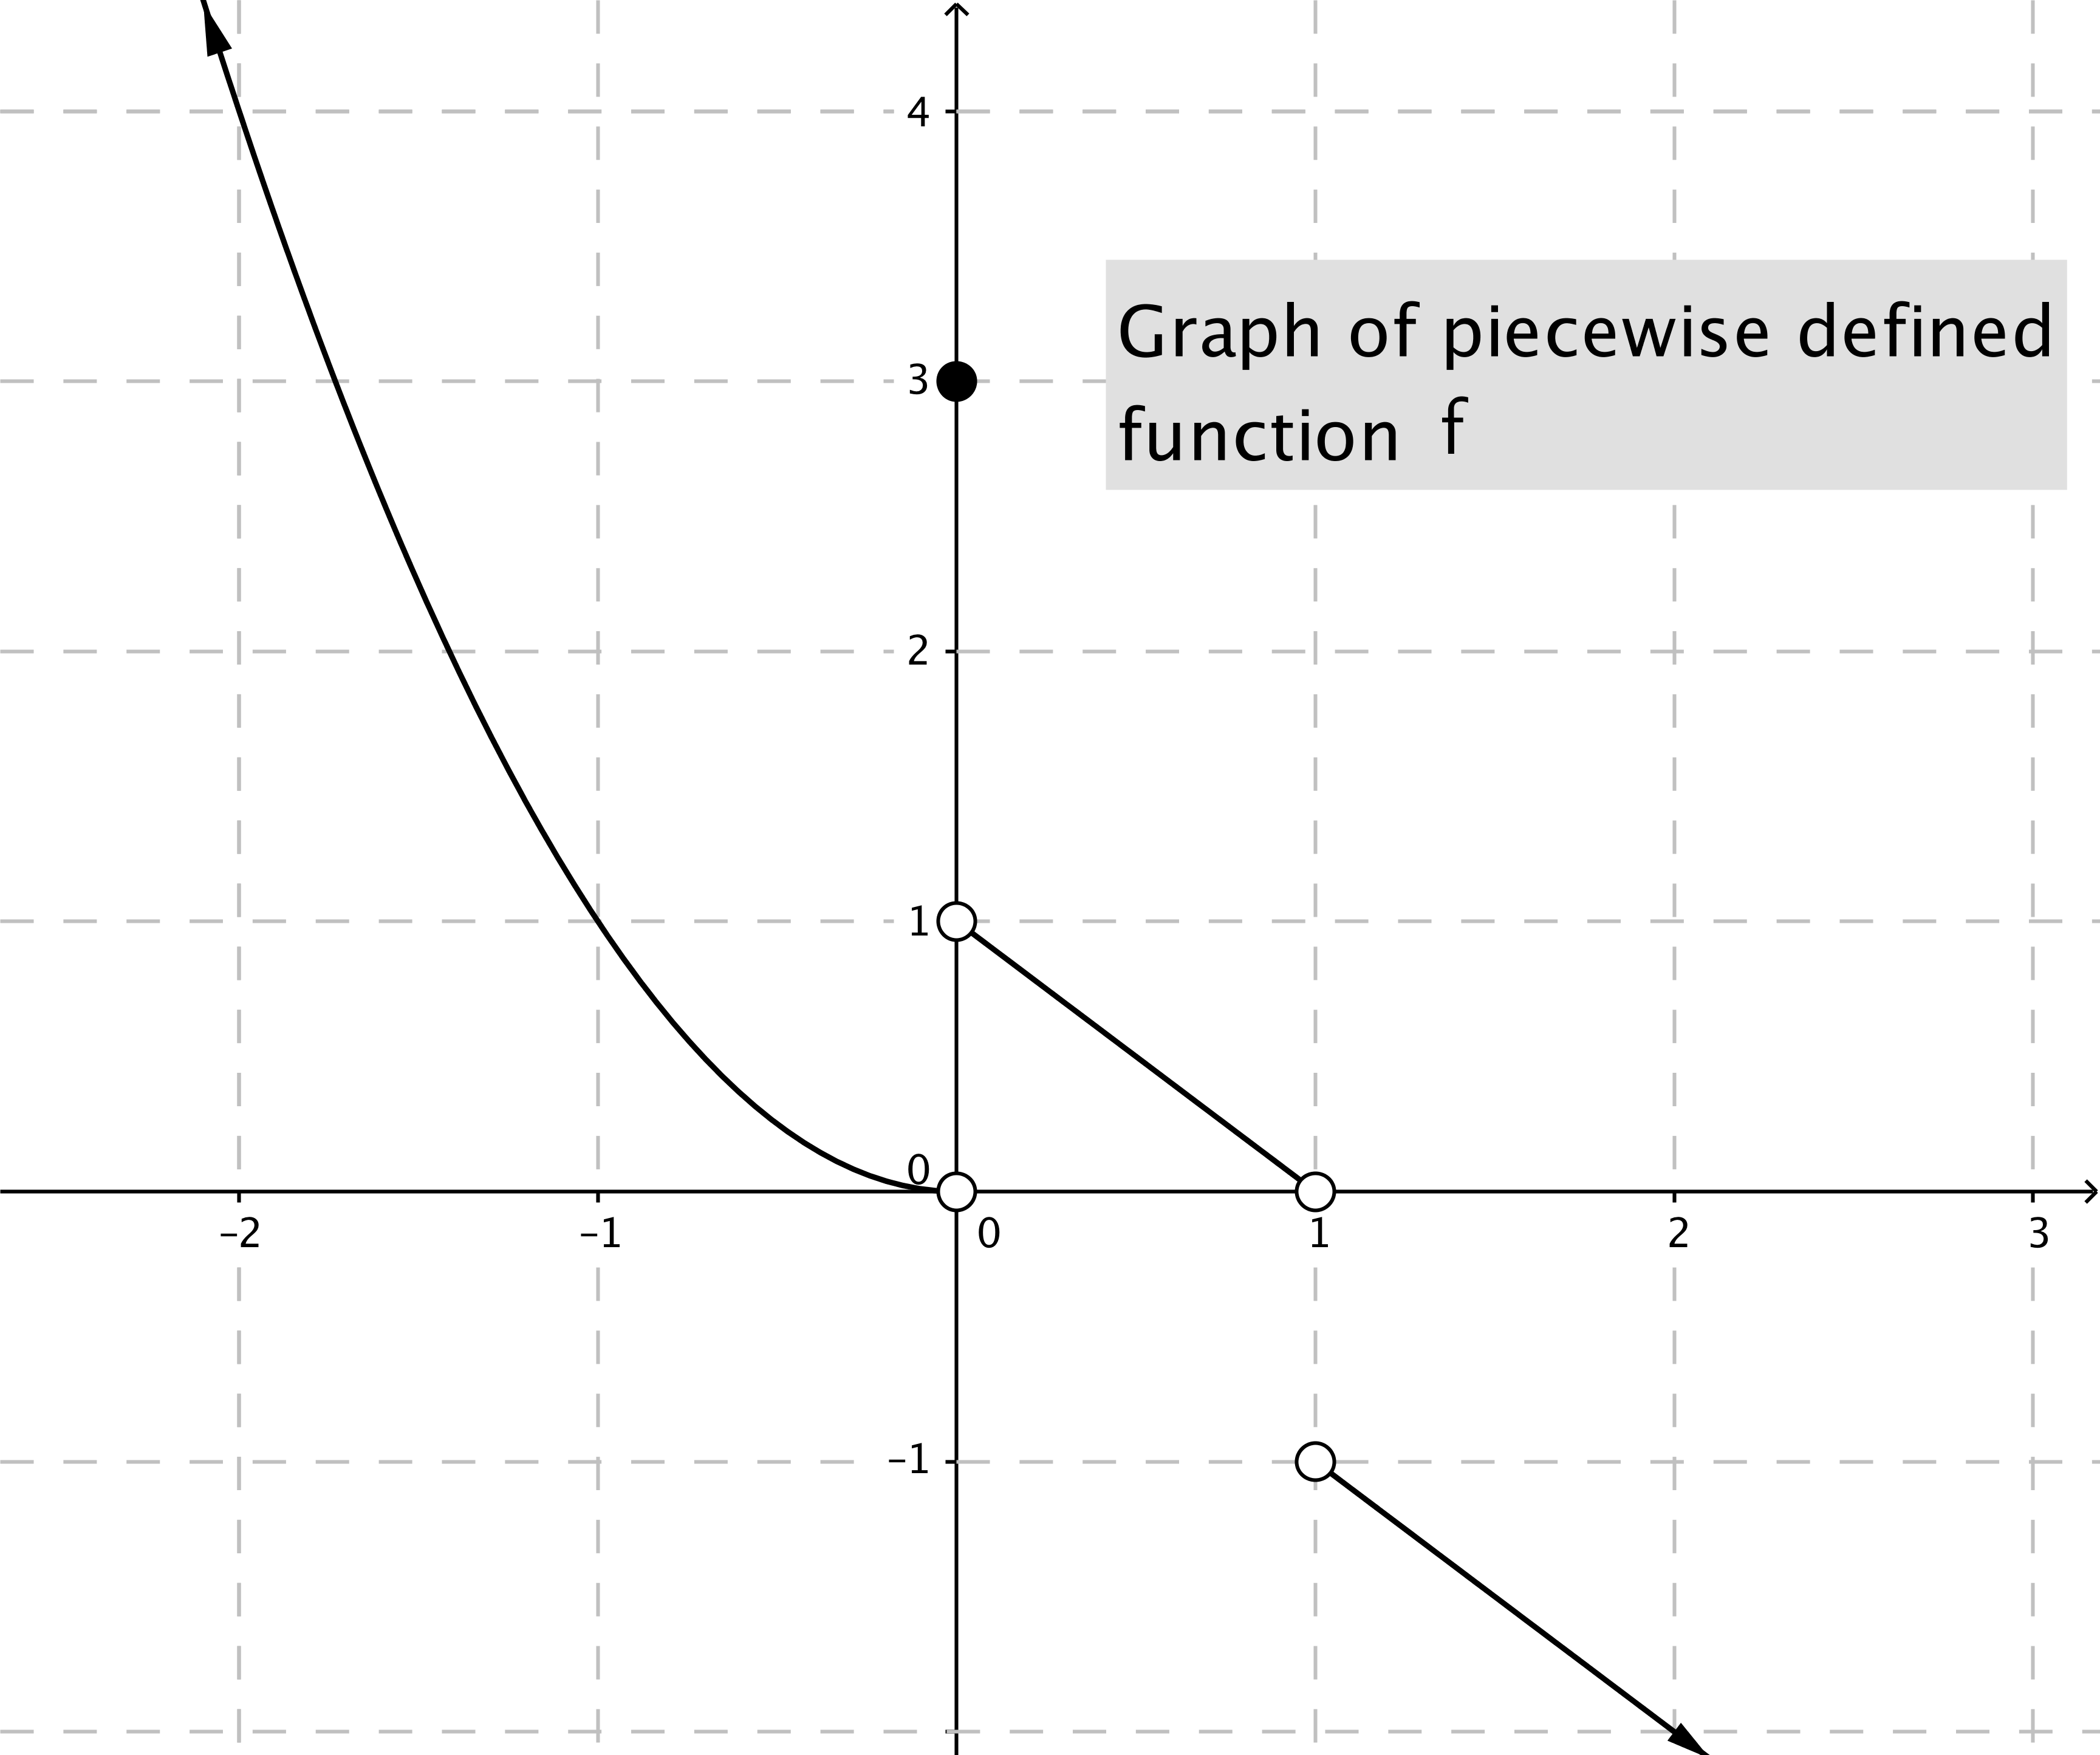
\includegraphics[scale = 0.3]{figure1.png}
  \end{image}
  Use this graph to answer the following questions:
  \begin{enumerate}
    \item
      What is the domain of this function?
      \begin{freeResponse}
        $(-\infty, 1) \cup (1, \infty)$
      \end{freeResponse}
      
    \item
      What is the range of this function?
      \begin{freeResponse}
        $(-\infty, -1) \cup (0, \infty)$
      \end{freeResponse}

    \item
      What is the value of $f(0)$, $f(1)$, and $f(2)$?
      \begin{freeResponse}
        $f(0) = 3$, $f(1)$ does not exist, $f(2) = -2$
      \end{freeResponse}

    \item
      Does this function have an inverse?
      (Why or why not?)
      \begin{freeResponse}
        No, the function does not have an inverse.
        It is not one-to-one (that is, it does not pass the horizontal line test).
      \end{freeResponse}
      
    \item
      Find at least two intervals on which the function is one-to-one.
      \begin{freeResponse}
        The function becomes one-to-one when we restrict its domain to $(-\infty, 0)$:
        \begin{image}
          \includegraphics[scale = 0.25]{"Graph of restricted function".png}
        \end{image}
        The function also becomes one-to-one when we restrict its domain to $[0, \infty)$:
        \begin{image}
          \includegraphics[scale = 0.5]{"Graph of second restricted function".png}
        \end{image}
      \end{freeResponse}

    \item
      Find $f^{-1}(3)$ on a restricted domain of $f$.
      \begin{freeResponse}
        In this case restrict the domain of $f$ to $[0, \infty)$.
        By definition we have $f^{-1}(3) = y \iff 3 = f(y)$.
        Looking at the second graph of the restricted function we see that $f(0) = 3$, that is, $f^{-1}(3) = 0$.

        (If we restric the domain of $f$ to $(-\infty, 0)$, then $f^{-1}(3) = y \iff 3 = f(y)$ implies that $f(-1.7) \approx 3$.
        Hence $-1.7 \approx f^{-1}(3)$.)
      \end{freeResponse}
  \end{enumerate}
\end{problem}

%problem3
\begin{problem}

  Let $g$ be a one-to-one function and let $g^{-1}$ be its inverse.
  \textbf{True or False:}
  If the point $(2, 1/5)$ lies on the graph of $g$, then the point $(2, 5)$ lies on the graph of $g^{-1}$.
  \begin{freeResponse}
    This statement is \textbf{false}: we have $g(2) = 1/5 \iff 2 = g^{-1}(1/5)$.
    The notation $g^{-1}$ never, in this course, means $1/g$.
  \end{freeResponse}
\end{problem}




%problem4
\begin{problem}
  Each of the following functions are invertible on their given domains.
  For each one find a formula for its inverse and give the domain and range of the inverse.
  \begin{enumerate}
    \item
      The function $f$ defined by $f(x)=x^2-4x-5$ for every $x \ge 2$.
      \begin{freeResponse}
        To help find the a formula for $f^{-1}$ we will first ``complete the square'':
        \begin{align*}
          x^2-4x-5 &= x^2 - 4x + 4 - 4 - 5,\\
                   &= (x - 2)^2 - 9.
        \end{align*}
    
        Setting $y = f(x) = x^2-4x-5 = (x - 2)^2 - 9$, we can follow the procedures outlined for algebracially finding the formula for an inverse function.
        \begin{align*}
          &\mbox{} y = (x - 2)^2 - 9\\
          &\implies y + 9 = (x - 2)^2\\
          &\implies \sqrt{y + 9} = |x - 2| \\
          &\implies \sqrt{y + 9} = x - 2 \hspace{1em} \mbox{(since $x \ge 2$)}\\
          &\implies \sqrt{y + 9} + 2 = x \\
          &\implies 2 + \sqrt{x + 9} = y \hspace{1em} \mbox{\parbox[b][]{6cm}{(interchange $x$ and $y$ along with minor rewriting)}}
        \end{align*}
        Therefore we have that $f^{-1}$ is defined by $f^{-1}(x) = 2 + \sqrt{x + 9}$.
        The domain of $f^{-1}(x)$ is $[-9, \infty)$ and the range is $[2, \infty)$.
      \end{freeResponse}

    \item
      The function $g$ defined by $g(u) = \sqrt[4]{u + 2}$.
      \begin{freeResponse}
        Following the procedure to algebraically find the formula for the inverse function we have
        \begin{align*}
          &\mbox{} z = \sqrt[4]{u + 2}\\
          &\implies z = (u+2)^{1/4}\\
          &\implies z^4 = u + 2\\
          &\implies z^4 - 2 = u\\
          &\implies u^4 - 2 = z \hspace{1em} \mbox{(interchange $u$ and $z$)}
        \end{align*}
        Therefore we have that $g^{-1}$ is defined by $g^{-1}(u) = u^4 - 2$.
        The domain of $g^{-1}$ is $[0, \infty)$ and the range is $[-2, \infty)$.
      \end{freeResponse}

    \item
      The function $h$ defined by $h(t) = 1/(t+2)^2$ for every $t > -2$.
      \begin{freeResponse}
        Following the procedure to algebraically find  the formula for the inverse function we have
        \begin{align*}
          &\mbox{} s = \frac{1}{(t+2)^2}\\
          &\implies (t+2)^2 = \frac{1}{s}\\
          &\implies |t + 2| = \sqrt{\frac{1}{s}} \\
          &\implies t + 2 = \sqrt{\frac{1}{s}} \hspace{1em} \mbox{(since $t > -2$)}\\
          &\implies t = \sqrt{\frac{1}{s}} - 2 \\
          &\implies s = \frac{1}{\sqrt{t}} - 2 \hspace{1em} \mbox{(interchange $s$ and $t$)}
        \end{align*}
        Therefore we have $h^{-1}$ is defined by $h^{-1} = \frac{1}{\sqrt{t}} - 2$.
        The domain of $h^{-1}$ is $(0, \infty)$ and the range is $(-2, \infty)$.
      \end{freeResponse}

    \item
      The function $p$ defined by $p(s) = e^{3s+1}$.
      \begin{freeResponse}
        Following the procedure to algebraically find  the formula for the inverse function we have
        \begin{align*}
          &\mbox{} y = e^{3s+1}\\
          &\implies \ln(y) = 3s + 1 \hspace{1em} \mbox{(since $\ln$ is the inverse of the natural exponential function)}\\
          &\implies \frac{\ln(y) - 1}{3} = s\\
          &\implies s = \frac{\ln(y) - 1}{3}\\
          &\implies y = \frac{\ln(s) - 1}{3} \hspace{1em} \mbox{(interchange $y$ and $s$)}
        \end{align*}
        Therefore we have $p^{-1}$ is defined by $p^{-1}(s) = (\ln(s) - 1)/3$.
        The domain of $p^{-1}$ is $(0, \infty)$ and the range is $(-\infty, \infty)$.
      \end{freeResponse}
  \end{enumerate}
\end{problem}

%problem5
\begin{problem}

  Find all real numbers $x$ which satisfy each of the following equations.
  \begin{enumerate}
    \item
      $\log_x 25 = 2$.
      \begin{freeResponse}
        Recall from that, by definition of the inverse to an exponential function,
        \[
        \log_b x = y \iff x = b^y.
        \]
        Using this relationship we have $\log_x 25 = 2 \iff x^2 = 25$.
        Therefore
        \begin{align*}
          x^2 = 25 &\implies x = \pm 5,\\
                   &\implies x = 5 \hspace{1em} \mbox{(base of log is always $>0$)}.
        \end{align*}
        Therefore $x = 5$ is the only solution to $\log_x 25 = 2$.
      \end{freeResponse}


    \item
      $7^x = 15$
      \begin{freeResponse}
        Similar to the previous problem,
        \[
        \log_b x = y \iff x = b^y .
        \]
        Using this relationship we have $7^x = 15  \iff x = \log_{7} 15$.
        Therefore $x = \log_7 15$ is the only solution to $7^x = 15$.
      \end{freeResponse}
      
    \item
      $\ln(x) + 1 = 0$.
      \begin{freeResponse}
        Similar to the previous two problems we'll use the relationship 
        \[
          \ln(x) = y \iff x = e^y.
        \]
        Before applying this relationship we perform a bit of algebra first:
        \[
          \ln(x) + 1 = 0 \implies \ln(x) = -1.
        \]
        Now we have $\ln(x) = -1 \iff x = e^{-1}$.
        Therefore $x = e^{-1} (= 1/e)$ is the only solution to $\ln(x) + 1 = 0$.
      \end{freeResponse}
  \end{enumerate}
\end{problem}

%problem1
\begin{problem}
  True or False:
  \begin{enumerate}
    \item[(1)]
      If $f(x) = (x-2)^x$, then $f'(x) = x (x-2)^{x-1}$.
      \begin{freeResponse}
        False.
        Any time that you have a function of $x$ raised to a function of $x$, in order to compute the derivative you need to use logarithmic differentiation (or something equivalent).

        Correct derivative of $f$:
        \begin{align*}
          f(x) &= (x-2)^x \implies f(x) = e^{x \ln(x-2)} \\
          &\implies f'(x) = e^{x \ln(x-2)} \cdot \left(1\cdot\ln(x-2) + x \cdot \frac{1}{x-2}\right) \\
          &\implies f'(x) = (x-2)^x \cdot \left(\ln(x-2) + \frac{x}{x-2}\right)
        \end{align*}
        \end{freeResponse}	
		
      \item[(2)]
        If $f(x) = (3x)^x$, then $f'(x) = (3x)^x \ln (3x)$.
	\begin{freeResponse}
          False.  Same as part (1).

          Correct derivative of $f$:
          \begin{align*}
            f(x) &= (3x)^x \implies f(x) = e^{x \cdot \ln(3x)} \\
            &\implies f'(x)  = e^{x \cdot \ln(3x)} \left(1 \cdot \ln(3x) + x \cdot \frac{3}{3x} \right) \\
            &\implies f'(x)  = (3x)^x \left(\ln(3x) + 1 \right)
          \end{align*}
	\end{freeResponse}	
	\end{enumerate}
\end{problem}

%problem2
\begin{problem}
Find the derivatives of the following functions:
	\begin{enumerate}
	
	%part a
	\item  $f(x) = x^{e^x} + 7x$
		\begin{freeResponse}
		$f'(x) = \ddx \left(x^{e^x} \right) + \ddx(7x) = \ddx \left(x^{e^x} \right) + 7$.  So the real problem is to find $\ddx \left(x^{e^x} \right)$.  
		
		\begin{align*}
		\ddx \left( x^{e^x} \right) &= \ddx \left( e^{\ln x^{e^x}} \right) \\
		&= \ddx \left( e^{e^x \ln x} \right) \\
		&= e^{e^x \ln x} \left( e^x \ln x + \frac{e^x}{x} \right) \\
		&= x^{e^x} \left( e^x \ln x + \frac{e^x}{x} \right).
		\end{align*}
		
		Thus, $f'(x) = x^{e^x} \left( e^x \ln x + \frac{e^x}{x} \right) + 7$.  
		
		\end{freeResponse}

	\item  $g(x) = (\ln x + 9)^{\sec(x^4)}$
		\begin{freeResponse}
			\begin{align*}
			g'(x) &= \ddx \left( (\ln x + 9)^{\sec(x^4)} \right) \\
			&= \ddx \left( e^{\sec(x^4) \ln ( \ln x + 9) } \right) \\
			&= e^{\sec(x^4) \ln ( \ln x + 9)} \left( 4x^3 \sec(x^4) \tan(x^4) \ln(\ln x + 9) + \sec(x^4) \frac{\frac{1}{x}}{\ln x + 9} \right) \\
			&= (\ln x + 9)^{\sec(x^4)} \left( 4x^3 \sec(x^4) \tan(x^4) \ln(\ln x + 9) + \frac{\sec(x^4)}{x(\ln x + 9)} \right) .
			\end{align*}
		\end{freeResponse}
		
	%part c
	\item  $h(x) = \frac{(x^2 - 7)^5}{\cos^7(x^2 - 5)}$
          \begin{freeResponse}
            Rewrite $h(x)$ using properties of logarithms:
            \begin{align*}
              \ln h(x) &= \ln \left( \frac{(x^2 - 7)^5}{\cos^7(x^2 - 5)}\right) \\
                       &= 5 \cdot \ln (x^2 - 7) + 7 \cdot \ln(\cos(x^2-5))
            \end{align*}
            % \begin{align*}
            %   h(x) &= e^{\ln(h(x))} = e^{\ln\left((x^2 - 7)^5/\cos^7(x^2 - 5)\right)}\\
            %   &= e^{\ln((x^2-7)^5) - \ln(\cos^7(x^2-5))} \\
            %   &= e^{5\cdot \ln((x^2-7)) - 7 \cdot \ln(\cos(x^2-5))}
            % \end{align*}

            Derivative of $h$:
            \begin{align*}
              \ddx \ln h(x) &\implies \frac{h'(x)}{h(x)} = 5 \cdot \frac{1}{x^2 - 7} \cdot 2x + 7 \cdot\frac{1}{\cos(x^2 - 5)} \cdot - \sin^2(x^2-5) \cdot 2x\\
                            &= \frac{10x}{x^2-7} - \frac{14x \cdot \sin(x^2 - 5)}{\cos(x^2 - 5)}\\
              &= \frac{10x}{x^2-7} - 14x \tan(x^2-5) \\
              &\implies h'(x) = h(x)\cdot \left( \frac{10x}{x^2-7} - 14x \tan(x^2-5) \right) \\
              &= h'(x) = \frac{(x^2 - 7)^5}{\cos^7(x^2 - 5)} \cdot \left( \frac{10x}{x^2-7} - 14x \tan(x^2-5) \right)
              % h(x) &= e^{5\cdot \ln((x^2-7)) - 7 \cdot \ln(\cos^7(x^2-5))}\\
              % &\implies h'(x) = e^{5\cdot \ln((x^2-7)) - 7 \cdot \ln(\cos(x^2-5))}\cdot \left(5\cdot \frac{1}{x^2-7} \cdot 2x - 7 \cdot -\sin(x^2-5)\cdot 2x \right) \\
              % &\implies h'(x) = h(x) \cdot \left( \frac{10x-35}{x^2-7} + 14x\sin(x^2-5)\right)
            \end{align*}
	\end{freeResponse}
	\end{enumerate}
\end{problem}






\end{document} 


















